\chapter{Chapter 3. Wavelet analysis as a single-spacecraft method}

Single-spacecraft measurements have been used in the identification of small-scale magnetic structures \citep{Pecora:2019, Telloni:2012, Hu:2018, Zheng:2018, Zhao:2020}. The time series data can be treated as a spatial snapshot due to the effective stationary state of the plasma medium traversed by a spacecraft relative to the fast-moving solar wind. Time series data are transformed directly to spatial distributions \citep{Taylor:1938}. Therefore, time-frequency transforms, such as wavelet transforms, are conceivably useful for analyzing features of in situ spacecraft time series at different frequencies over time \citep{Torrence:1998}. Specifically the power spectra associated with a number of selected MHD quantities are derived to characterize the underlying magnetic structures.

\section{Wavelet transforms}
Wavelet transforms are used to analyze time series with non-stationary power at different frequencies \citep{Torrence:1998} using non-orthogonal wavelet basis functions. Assuming a continuous signal as a function of time $t$, $x=x(t)$, the continuous wavelet transform is defined as
\begin{equation}
    W(s,\tau) = \frac{1}{|s|^{1/2}}\int_{-\infty}^\infty x(t)\psi^*\p{\frac{t-\tau}{s}}\textnormal{dt}.
    \label{eq:wavetrans}
\end{equation}
Here $\psi^*$ is the complex conjugate of the wavelet basis function $\psi(t)$, which is a function that must be localized in time and frequency space, and has zero mean \citep{Torrence:1998}.

As usual, with a discrete set of data points $x_n=x(t_n)$ with time resolution $\delta t$, the continuous wavelet transform takes the discrete form
\begin{equation}
    W_n(s,t) = \sum_{n'=0}^{N-1}x_{n'}\psi^*\pp{\frac{\p{n'-n}\delta t}{s}}.
    \label{eq:wavetrans2}
\end{equation}
In practice, discrete wavelet transforms are implemented for time series data by dilating the scale $s$ and translating along the time index $n$. This results in a two dimensional array of the wavelet transform. The scales are chosen such that
\begin{equation}
    J = \frac{\log_2\p{\frac{N \delta t}{s_0}}}{dj}
\end{equation}
\begin{equation}
    s_j = s_0 2^{j dj},\hspace{20pt} j = 0,...,J
    \label{eq:scales}
\end{equation}
where $s_0 = 2\delta t$ and the choice of $dj$ is sufficiently small for the width of the wavelet basis function in spectral space. The Morlet wavelet given in Equation (\ref{eq:morlet}) is a good wavelet base because it is complex and has good frequency resolution, thus it is frequently used in small-scale flux rope identification \citep{Telloni:2012, Telloni:2013, Zhao:2020, Farge:1992}:
\begin{equation}
    \psi_0(\eta) = \pi^{-1/4}e^{i\omega_0\eta}e^{-\eta^2/2}.
    \label{eq:morlet}
\end{equation}

Figure \ref{fig:wavelet-diagram} visually demonstrates the typical transform of a time series data set from the time domain to a time-frequency domain, including the Fourier transform and the wavelet transform. Wavelet transforms take a one-dimensional time series (top left corner of Figure \ref{fig:wavelet-diagram}) and transform it into a two-dimensional series (bottom right corner of Figure \ref{fig:wavelet-diagram}), whereas the Fourier transform applied to a one-dimensional time series yields a one-dimensional series in the frequency domain (top right corner of Figure \ref{fig:wavelet-diagram}). The Fourier transform decomposes a time series function into a combination of the frequencies present in the data set \citep{Farge:1992}. The Fourier transform of a time series $x(t)$ into its frequency domain (index $k$) is
\begin{equation}
    F(k) = \int_{-\infty}^\infty x(t) e^{-2\pi ikt/N} \textnormal{dt},
    \label{eq:fourier}
\end{equation}
\noindent and with discrete data $x_n = x(t_n)$, it takes the form
\begin{equation}
    F_n(k) = \frac{1}{N} \sum_{n=0}^{N-1}x_{n} e^{-2\pi ikn/N}.
    \label{eq:DFT}
\end{equation}
A short time Fourier transform (bottom left corner of Figure \ref{fig:wavelet-diagram}) can produce a two-dimensional time-frequency domain, but by segmenting the time series and performing a Fourier transform over the segments, the method only yields identical time-frequency domains, for each respective time segment. Fourier transforms theoretically retain all the `information' about an equation, but discrete Fourier transforms are a summation over a finite set and therefore are not as accurate. 

\begin{figure}
    \centering
    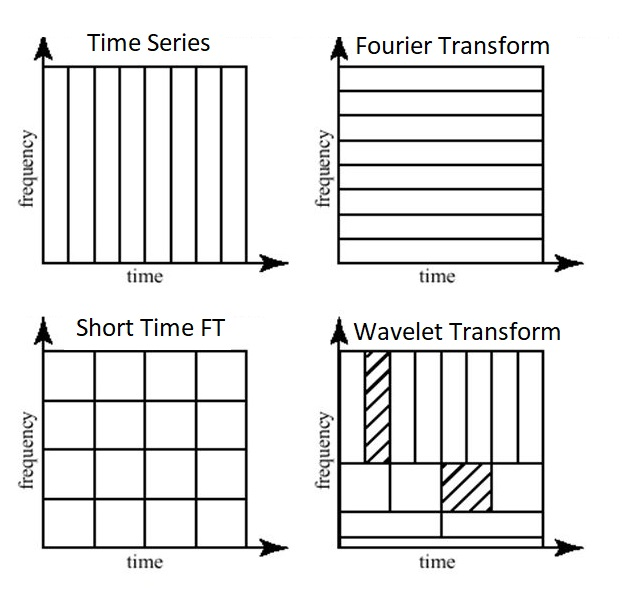
\includegraphics[width=0.7\textwidth]{Figures/Comparisonoftransformations.jpeg}
    \caption[Time and frequency resolutions of different transforms]{Time and frequency resolutions of different transforms applied to a one-dimensional time series dataset. The wavelet transform (bottom right) has non-uniform frequency and time resolution.}
    \label{fig:wavelet-diagram}
\end{figure}

% The calculation in (\ref{eq:wavetrans2}) can be more efficiently done in Fourier space. Using a discrete Fourier transform, all $N$ convolutions can be done simultaneously for each scale $s$. The discrete Fourier transforms of the time series $\xhat_k=x_n$ and $\psihat^*(s\omega_k)=\psi^*(s,t)$ are
% \eql{DFT}{\xhat_k = \frac{1}{N}\sum_{n=0}^{N-1}x_n e^{-2\pi ikn/N}}

% \eql{DFTpsi}{}

% By the convolution theorem, a wavelet transform is inverse Fourier transform of the product
% \eql{wavelet}{W_n(s,t) =\sum_{k=0}^{N-1} \xhat_k \psihat^*\p{s\omega_k} e^{i\omega_k n\delta t}}
% where

\section{MHD quantities}
The magnetic field lines in flux ropes are twisted such that they preside in a tube-like configuration. Thus, flux ropes carry magnetohydrodynamic (MHD) quantities such as cross helicity $H_c$ and magnetic helicity $H_m$, as well as residual energy $E_r$, defined as
\begin{equation}
    H_c = \frac{1}{2}\int \mathbf{v}\cdot\mathbf{b} \hspace{5pt} \mathrm{d^3} \mathbf{r}
    \label{eq:Hc}
\end{equation}
\begin{equation}
    H_m = \int \mathbf{A}\cdot\mathbf{B} \hspace{5pt} \mathrm{d^3} \mathbf{r}
    \label{eq:Hm}
\end{equation}
\begin{equation}
    E_r = \frac{1}{2} \pp{\pang{\mathbf{v}^2}  - \pang{\mathbf{b}^2}},
    \label{eq:Er}
\end{equation}
where $\mathbf{B}\p{\mathbf{x},t}$ is the magnetic field, $\mathbf{A}\p{\mathbf{x},t}$ is the magnetic vector potential, and $\mathbf{v}(\mathbf{x},t)$ and $\mathbf{b}(\mathbf{x},t)$ are the fluctuating velocity and magnetic field in Alfv\'en units. Cross helicity describes the measure of alignment between magnetic and velocity fluctuations, while magnetic helicity describes the “knottedness” of the magnetic field lines \citep{Matthaeus:1982}. High magnetic helicity is a signature of flux ropes, and often accompanied by low cross helicity \citep{Zhao:2020}. Residual energy describes the imbalance between magnetic and kinetic energy, and thus according to (\ref{eq:Er}), a negative residual energy will characterize an event with higher magnetic energy.
%When normalized, these magnetohydrodynamic quantities give insight into the nature of magnetic field structures, and allow us to identify these events in the solar wind and Earth's magnetosphere.

Normalized MHD quantities give insight into the nature of magnetic field structures, and allow us to identify and characterize these events. Approximated in the time domain, the normalized cross helicity and residual energy can be calculated using
\eql{eq:sigctime}{\sigma_c = \frac{2\langle\mathbf{v}\cdot\mathbf{b}\rangle}{\langle\mathbf{v}^2\rangle + \langle\mathbf{b}^2\rangle}}
\eql{eq:sigrtime}{\sigma_r = \frac{\langle\mathbf{v}^2\rangle - \langle\mathbf{b}^2\rangle}{\langle\mathbf{v}^2\rangle + \langle\mathbf{b}^2\rangle}}
where $\mathbf{v}$ is the remaining flow in the de Hoffman-Teller frame. Single spacecraft measurements cannot be used directly calculate reduced magnetic helicity, therefore other methods are required to approximate this quantity. The power spectral density of a time series describes the distribution of the energy across the frequency components of a signal. \cite{Matthaeus:1982} showed that a form of the magnetic helicity can be calculated using single spacecraft measurements by utilizing the power spectral density. This can often be done in a similar fashion using wavelet transforms \citep{Telloni:2012, Telloni:2013}. The continuous wavelet transform of a one-dimensional time series yields the two-dimensional time-scale spectrogram for a finite time period. This shows how the amplitude of a feature versus the scale varies with time, therefore making it useful in studying the features associated with multi-scale structures. The so-called reduced form of the magnetic helicity gives quantitative information about the magnetic helicity density along the radial dimension, $X$, and is calculated with Fourier transforms of the $Y$- and $Z$-components of the magnetic field, $\tilde F(B_Y)$ and $\tilde F(B_Z)$,
\begin{equation}
    H_m(k) = \frac{2 \textnormal{Im}\left[S_{YZ} (k)\right]}{k} = \frac{2 \textnormal{Im}\pp{\tilde F^*(B_Y)\tilde F(B_Z)}}{k},
\end{equation}
where $S_{YZ}(k)$ is one element of the reduced magnetic power spectral density tensor \citep{Matthaeus:1982}. \cite{Telloni:2012} showed that taking $X$ along the radial direction from the sun, wavelet transforms of the magnetic field $Y$- and $Z$-components, the Els\"asser variables $Z^\pm$, and kinetic and magnetic energies enable an efficient way to calculate the reduced normalized magnetic helicity \gls{sigma_m}, cross helicity \gls{sigma_c}, and residual energy \gls{sigma_r}, corresponding to equations (\ref{eq:Hc})-(\ref{eq:Er}):
\begin{equation}
    \sigma_m(k,t) = 2\frac{\textnormal{Im}\left[W_Y(k,t)W_Z^*(k,t)\right]}{|W_X(k,t)|^2 + |W_Y(k,t)|^2 + |W_Z(k,t)|^2} ,
    \label{eq:sigm}
\end{equation}
\begin{equation}
    \sigma_c(k,t) = \frac{W^+(k,t)-W^-(k,t)}{W^+(k,t)+W^-(k,t)} ,
    \label{eq:sigc}
\end{equation}
 \begin{equation}
    \sigma_r(k,t) = \frac{W_{kin}(k,t) - W_{mag}(k,t)}{W_{kin}(k,t) + W_{mag}(k,t)} .
    \label{eq:sigr}
\end{equation}

\noindent Here $W_X(k,t),W_Y(k,t),W_Z(k,t),W^+(k,t)$, and $W^-(k,t)$ are the wavelet transforms of $B_X,B_Y,B_Z,Z^+$, and $Z^-$, respectively. The Els\"asser variables, $Z^\pm = \mathbf{v} \pm \mathbf{b}$, are the combination of the velocity and magnetic field fluctuations in Alfv\'en units. $W_{kin}(k,t)$ and $W_{mag}(k,t)$ are the sums of the power of the wavelet transforms of the components of the velocity and magnetic field (in Alfv\'en units). Equations (\ref{eq:sigm})-(\ref{eq:sigr}) can also be written in terms of scale and time : %by multiplying the numerator and denominator by $V_0 = \frac{2\pi}{k}$,
\begin{equation}
    \sigma_m(s,t) = 2\frac{ V_{X0}\textnormal{Im}\pp{W_Y(s,t)W_Z^*(s,t)}}{V_0 \p{|W_X(s,t)|^2 + |W_Y(s,t)|^2 + |W_Z(s,t)|^2}}, %+ V_{Y0}\textnormal{Im}\pp{\tilde F^*(B_Z)\tilde F(B_X)} + V_{Z0}\textnormal{Im}\pp{\tilde F^*(B_X)\tilde F(B_Y)}
    \label{eq:sigm-st}
\end{equation}
\begin{equation}
    \sigma_c(s,t) = \frac{W^+(s,t)-W^-(s,t)}{W^+(s,t)+W^-(s,t)} ,
\end{equation}
 \begin{equation}
    \sigma_r(s,t) = \frac{W_{kin}(s,t) - W_{mag}(k,t)}{W_{kin}(s,t) + W_{mag}(s,t)} .
\end{equation}
since $\kvec \parallel \Vvec_0$ \citep{Zhao:2021, Horbury:2008, Taylor:1938}, where $\Vvec_0$ is the average plasma velocity. Equation \ref{eq:sigm-st} only shows the first term of the trace of the power spectrum because the radial component is dominant over the tangential component at 1 AU.


% \begin{equation}
%   \label{example}
%   \begin{split}
%    \nabla \cdot \nabla \psi &= \frac{\partial^2 \psi}{\partial x^2} + \frac{\partial^2 \psi}{\partial y^2} + \frac{\partial^2 \psi}{\partial z^2} \\
%    &= \frac{1}{r^2 \sin\theta} \left[ \sin\theta \left( r^2 \frac{\partial \psi}{\partial r} \right) + \frac{\partial}{\partial \theta} \left( \sin \theta  \frac{\partial \psi}{\partial r} \right) + \frac{1}{\sin \theta} \frac{\partial^2 \psi}{\partial \varphi^2}  \right] 
%      \end{split}
% \end{equation}

\section{Algorithm for identification of magnetic structures} \label{sec:wavelet-algorithm}
In Figure \ref{fig:wavelet-spectrograms-mms}, the time series of the magnetic field and plasma parameters from 10:20-13:30 UT on 9 November 2019 are shown. Panels (a) and (b) show the magnetic field and velocity components of the time period, with magnetic field magnitude reaching a maximum of about 20 nT and a flow velocity deflected from the Sun-Earth direction. Panel (c) shows relatively high proton density, varying from 20 to 30 cm$^{-3}$, and proton temperature of 1-2$\times 10^{6}$ K, which is typical for magnetosheath plasma. Panel (d) shows the Alfv\'en speed and the bulk plasma speed with a mean value for this 3 hour period (193 km/s) subtracted. Panel (e) shows the proton beta, which is between approximately 1-100. Panel (f) of Figure \ref{fig:wavelet-spectrograms-mms} displays the spectrogram reduced magnetic helicity, which describes the “knottedness” of the magnetic field lines. Panel (g) shows the normalized measure of alignment between magnetic and velocity fluctuations, reduced cross helicity, and panel (h) shows the imbalance between magnetic and kinetic energy, or reduced residual energy \citep{Matthaeus:1982}. These spectrograms show how the reduced MHD quantities vary in time and frequency, thus allowing us to search them for characteristics that are distinctive to different types of magnetic structures.

\begin{figure}
    \centering
    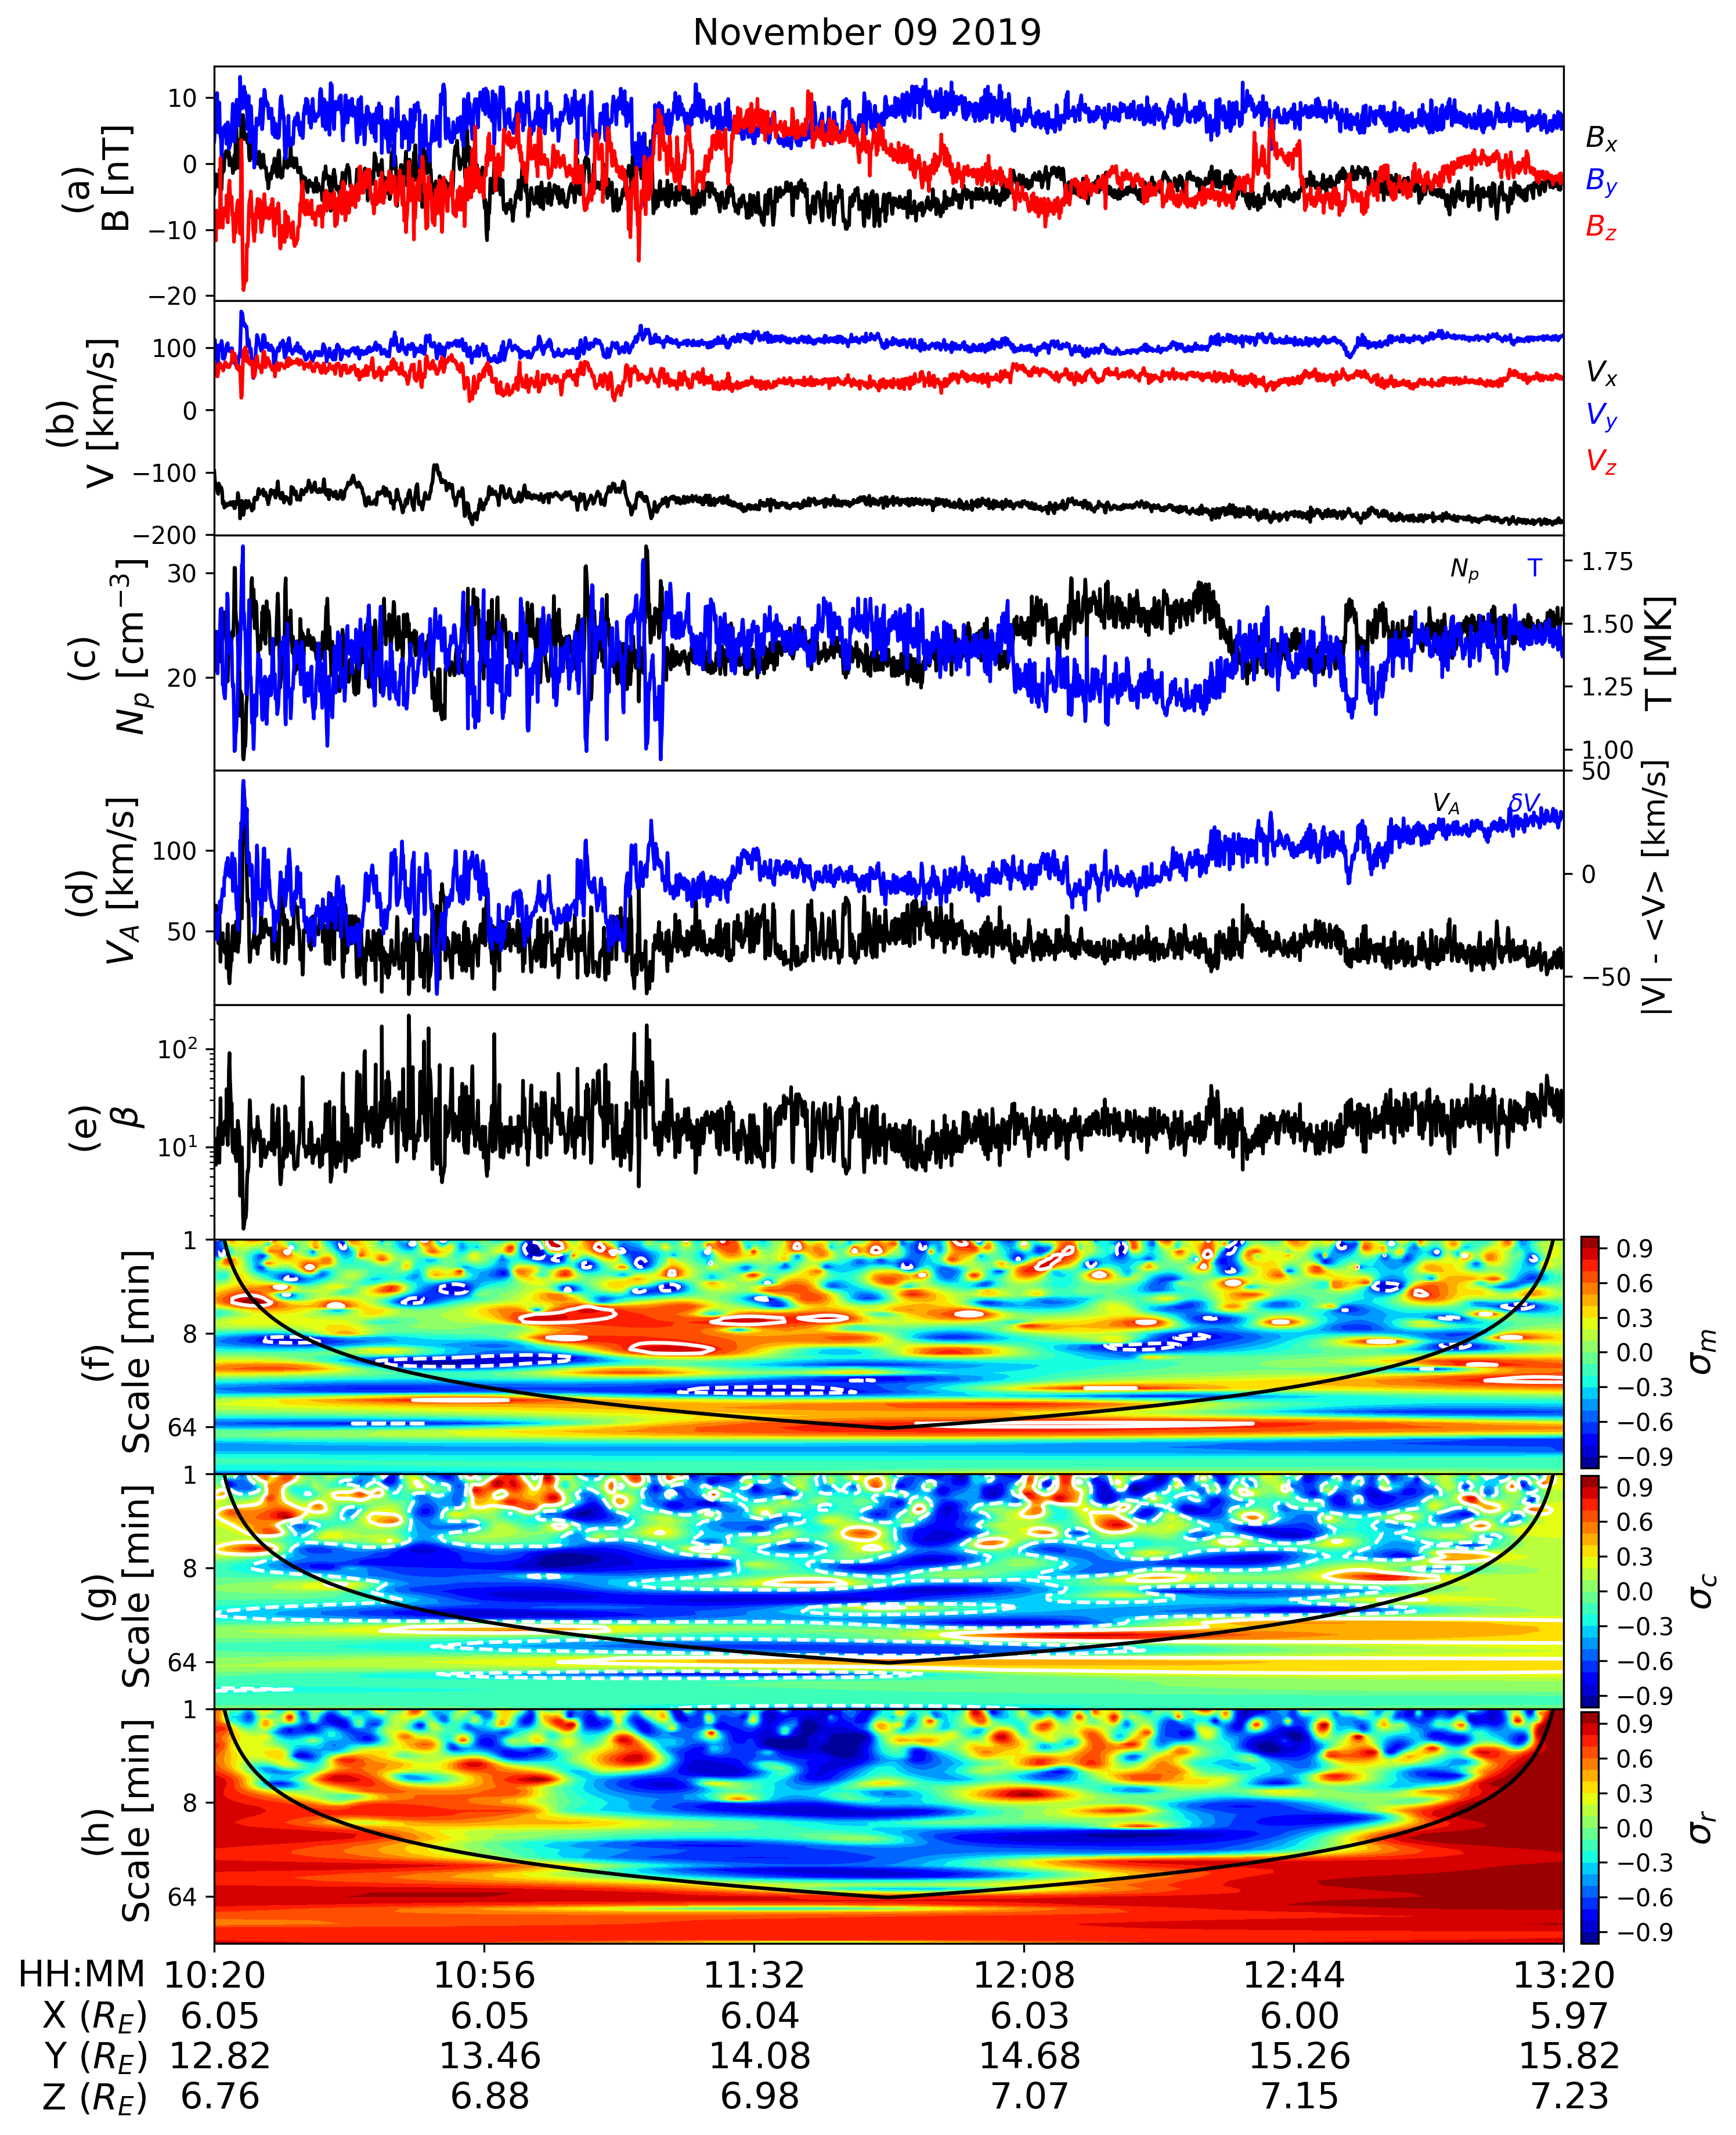
\includegraphics[width=0.8\textwidth]{Figures/Time series/spectrograms_09112019_1020_MMS1.png}
    \caption[Time series data and spectrograms of MHD quantities for 9 November 2019]{Time series of (a) magnetic field, (b) velocity, (c) plasma density and temperature, (d) Alfv\'en speed and velocity fluctuations, (e) plasma beta, and spectrograms of the normalized (f) reduced magnetic helicity, (g) cross helicity, and (h) residual energy found by wavelet analysis, across multiples scales (as indicated by the vertical axes), during a 3 hour period that MMS-1 was in the magnetosheath on 9 November 2019. White contours in panel (f) and (g) represent regions of high reduced magnetic helicity ($|\sigma_m| \geq 0.75$) and regions of low reduced cross helicity ($|\sigma_c| \leq 0.3$), respectively. The black curved line in panels (f)-(h) is the cone of influence.}
    \label{fig:wavelet-spectrograms-mms}
\end{figure}

Structures with local enhanced magnetic helicity are identified with specific criteria: (i) magnetic helicity with absolute values greater than 0.75, (ii) duration between 30 seconds and 3 hours, and (iii) if the event was within the cone of influence, which arises because of finite data segment length \citep{Torrence:1998}. I calculate reduced, normalized forms of magnetic helicity $\sigma_m$, cross helicity $\sigma_c$, and residual energy $\sigma_r$ in 2400-point windows ($\sim$3 hours for MMS and $\sim$2 hours for THEMIS) across the hours-long periods identified in the solar wind and magnetosheath. Figure \ref{fig:spectrograms-interval} displays the spectrograms of reduced magnetic helicity from 10:20-13:30 UT and 11:05-14:05 UT on 9 November 2019. These intervals are calculated from the time series in Figure \ref{fig:wavelet-spectrograms-mms}. Events identified with the wavelet analysis method are marked with a grey interval. The black contours represent event candidates with $|\sigma_m|\geq 0.75$ whereas the white contours indicate events that were established in the final event list. Inside the white contours, a white ``X" marks the absolute local maximum, and the yellow annotations and dashed lines indicate the scale corresponding to a maximum. This scale is taken as the duration of the event, and the time of the peak in reduced $\sigma_c$ is taken to the time-wise midpoint of the event. Therefore, the event interval start time will be the time of the peak in $|\sigma_m|$ minus half of the scale size of the peak. The events identified from this wavelet analysis can be further characterized by implementing the criteria that the events have (iv) corresponding cross helicity with absolute value less than 0.3, to ensure that there is low level of velocity fluctuations and/or (v) negative residual energy, which indicates that the magnetic energy is dominant.
\begin{figure}
    \centering
    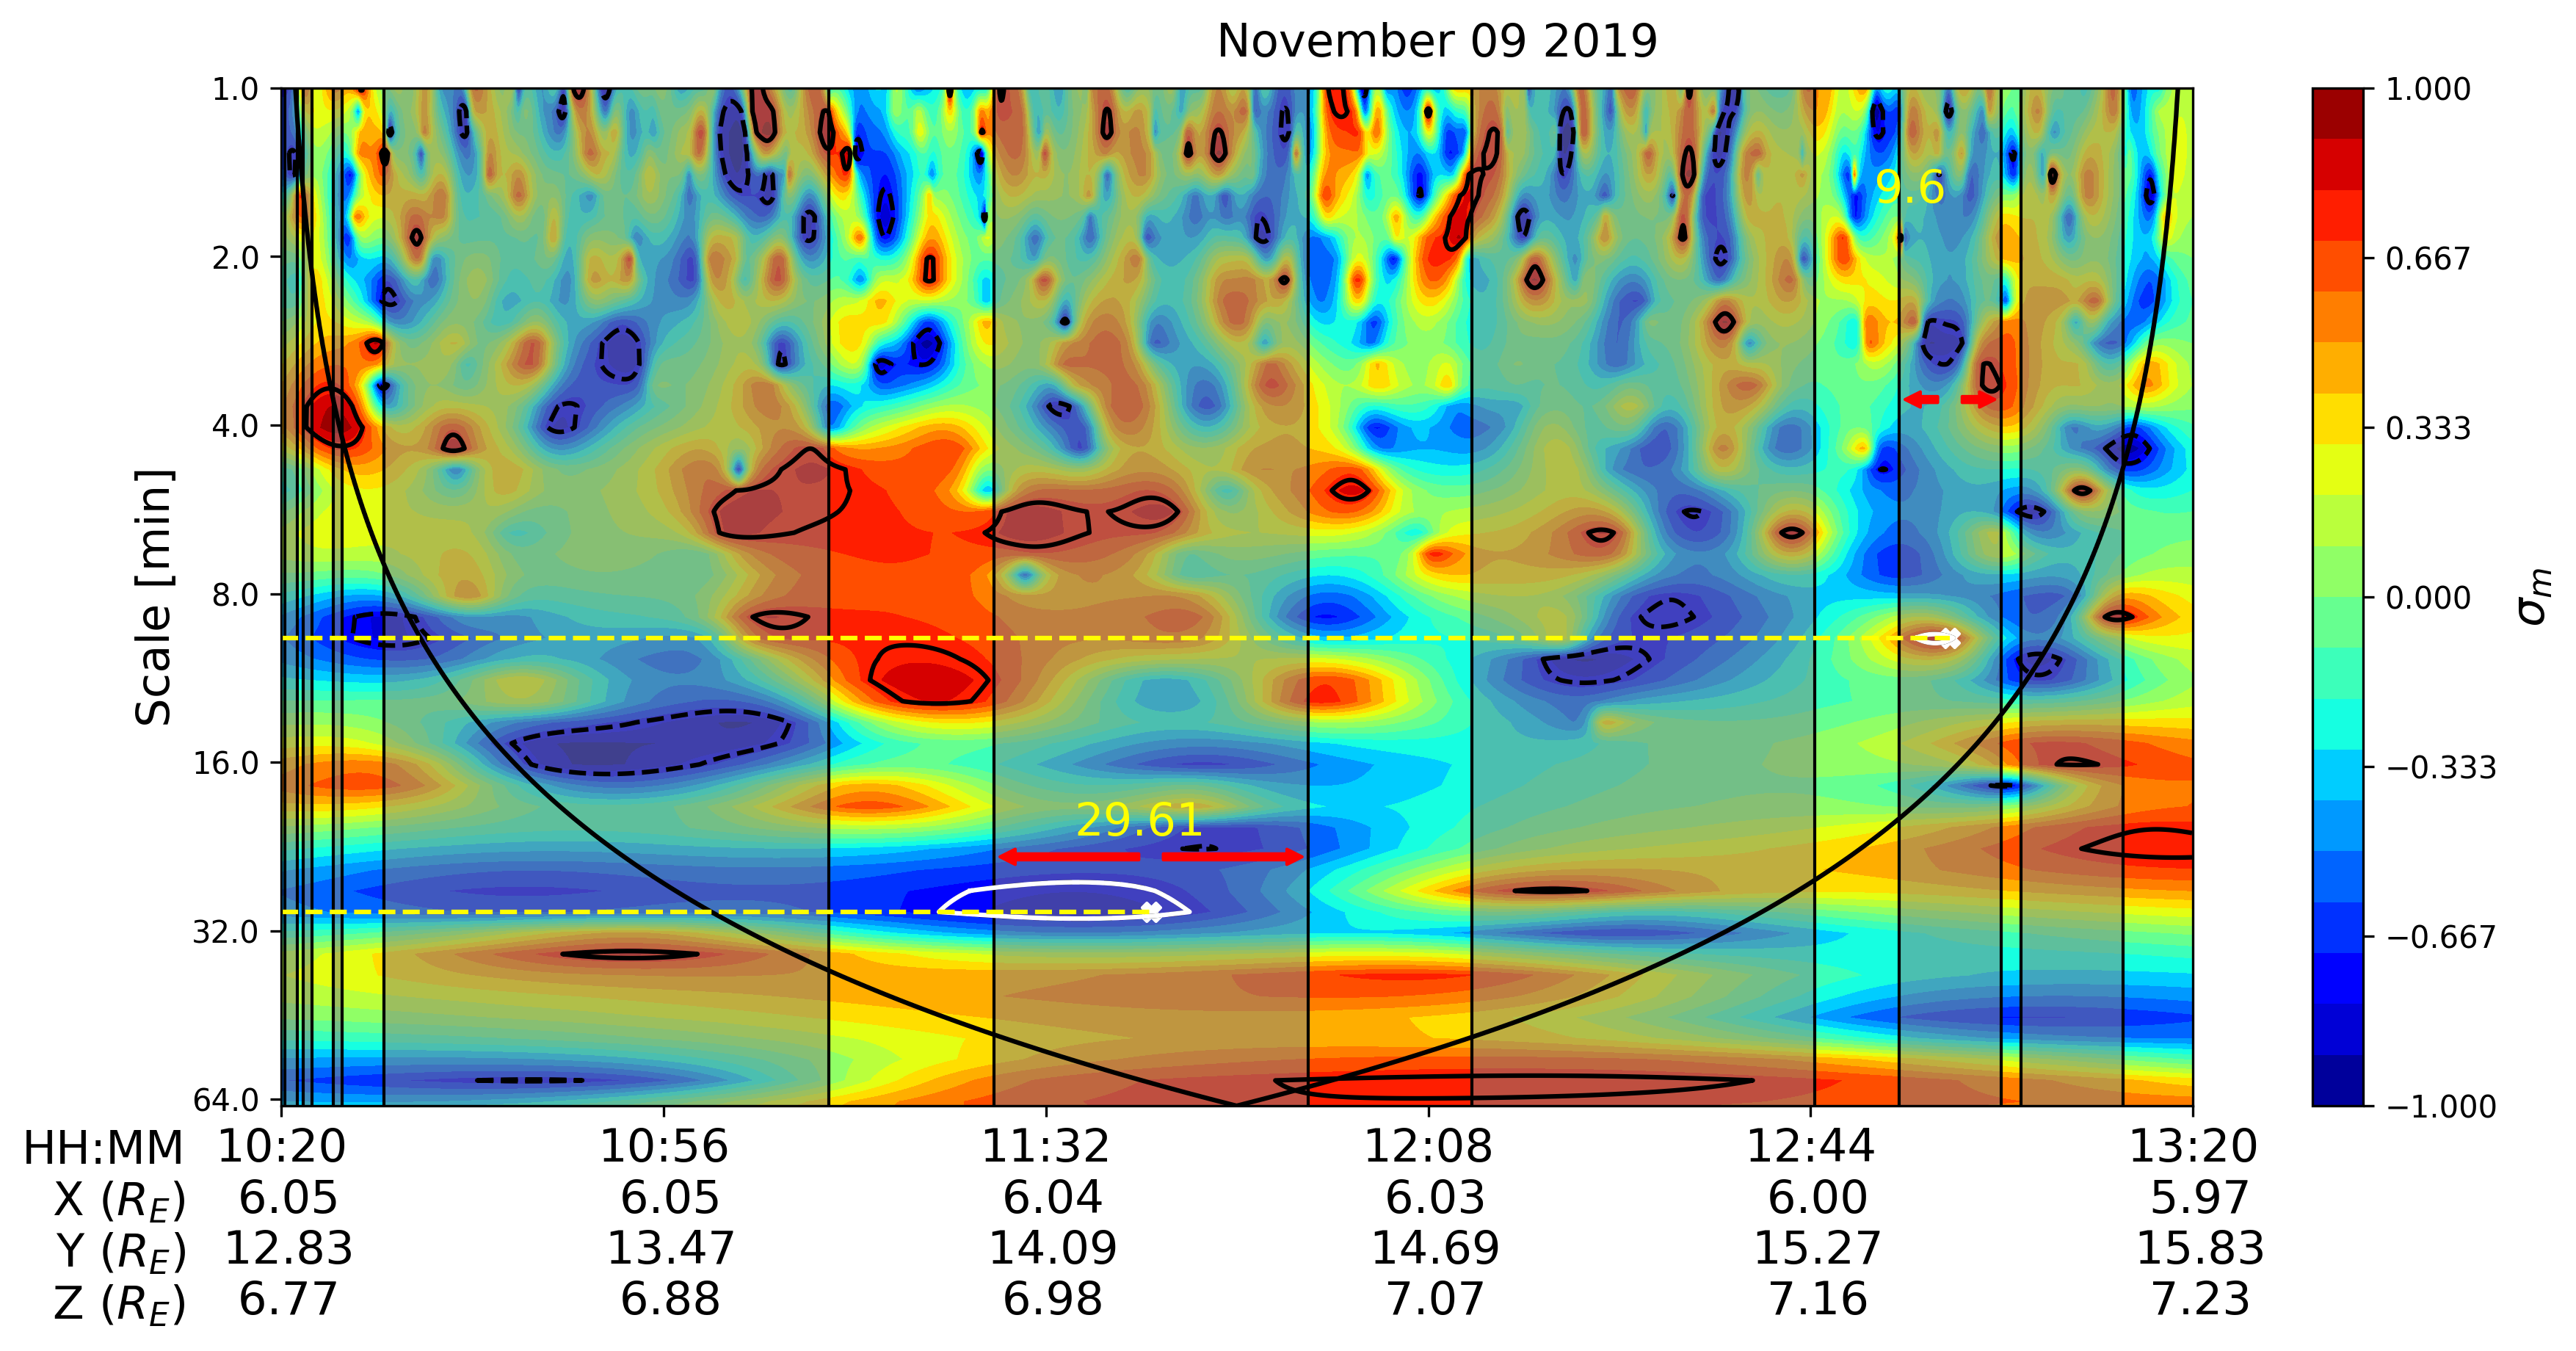
\includegraphics[width=\textwidth]{Figures/Spectrograms/magnetichelicity_wave_events_09112019_1020.png}
    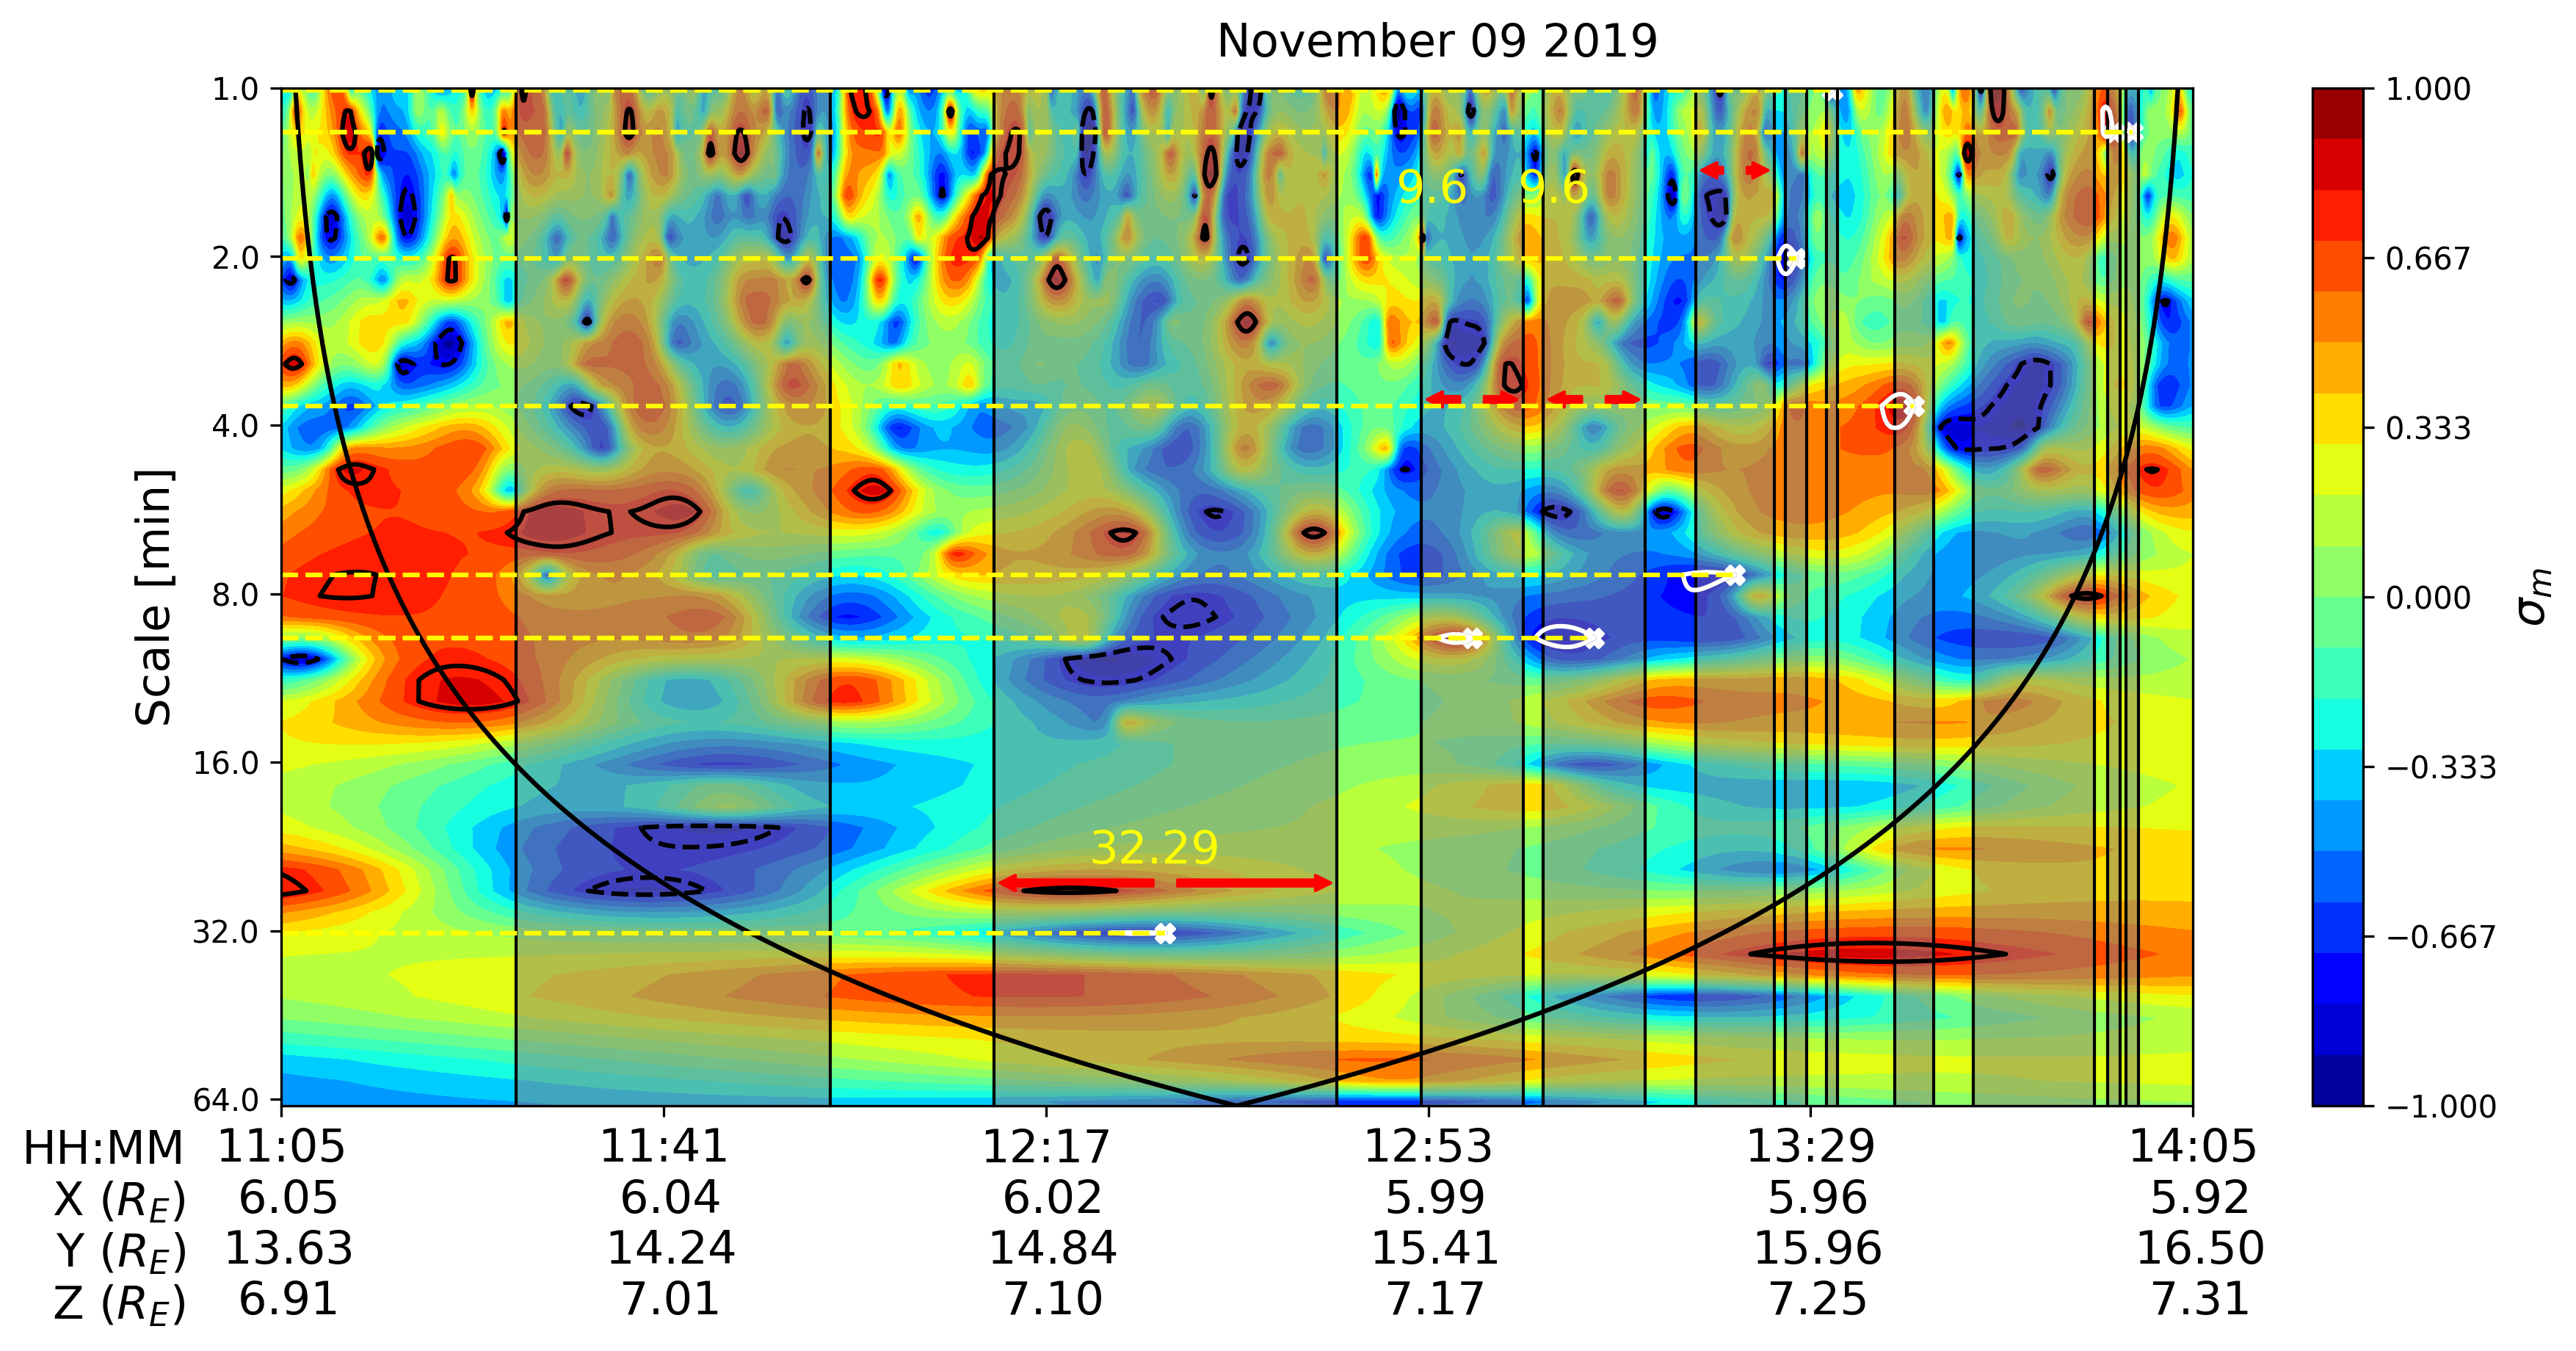
\includegraphics[width=\textwidth]{Figures/Spectrograms/magnetichelicity_wave_events_09112019_1105.png}
    \caption[Diagram of wavelet analysis identification algorithm via spectrograms of MHD quantities]{Spectrograms of reduced magnetic helicity over two overlapping 3-hour period from MMS-1 data on 9 November 2019. Demarcated intervals are identified events via wavelet analysis. Black contours represent regions of high reduced magnetic helicity ($|\sigma_m| \geq 0.75$). White contours represent regions of $|\sigma_m| \geq 0.75$ where the maximum inside the contour is an established event. Yellow dashed lines connect the maximum of the contour to the x-axis (scale) of the maximum. Red arrows indicate half of the scale (duration) on either side of the peak of $\sigma_c$. The black curved line is the cone of influence.}
    \label{fig:spectrograms-interval}
\end{figure}

It can be seen that not all grey event intervals have a white contour and marker for the maximum $\sigma_c$. This is because of the windowed analysis: as the maxima in reduced magnetic helicity are recorded in each window, there will be overlapping events identified. The intervals in Figure \ref{fig:spectrograms-interval} are overlapping by 600 data points (45 minutes for MMS data). After all the windows are searched, the compiled event list is then processed to eliminate overlapping events. By comparing two adjacently overlapping events and keeping the one with the highest maximum $|\sigma_m|$, this is repeated until there are no overlapping events left. Figure \ref{fig:wavelet-spectrograms-interval} shows an example of event intervals identified via the wavelet algorithm (with the criteria $|\sigma_m|\geq 0.75$) overlaid the corresponding time series and spectrogram of the reduced magnetic helicity in the magnetosheath during 9 November 2019. There are 11 events identified by the wavelet algorithm during this 3 hour period. The duration of these events range from 1 minute to 32.29 minutes, with an average duration of 9.913 minutes. The average maximum magnetic field of the events is 12.23 nT. The average absolute maximum (normalized) magnetic helicity of these 11 events is 0.83. 6 events in this period have $|\sigma_c|\leq 0.3$, and one of those events has $\sigma_r<0$. Of remaining 5 events, none have $\sigma_r<0$.

\begin{figure}
    \centering
    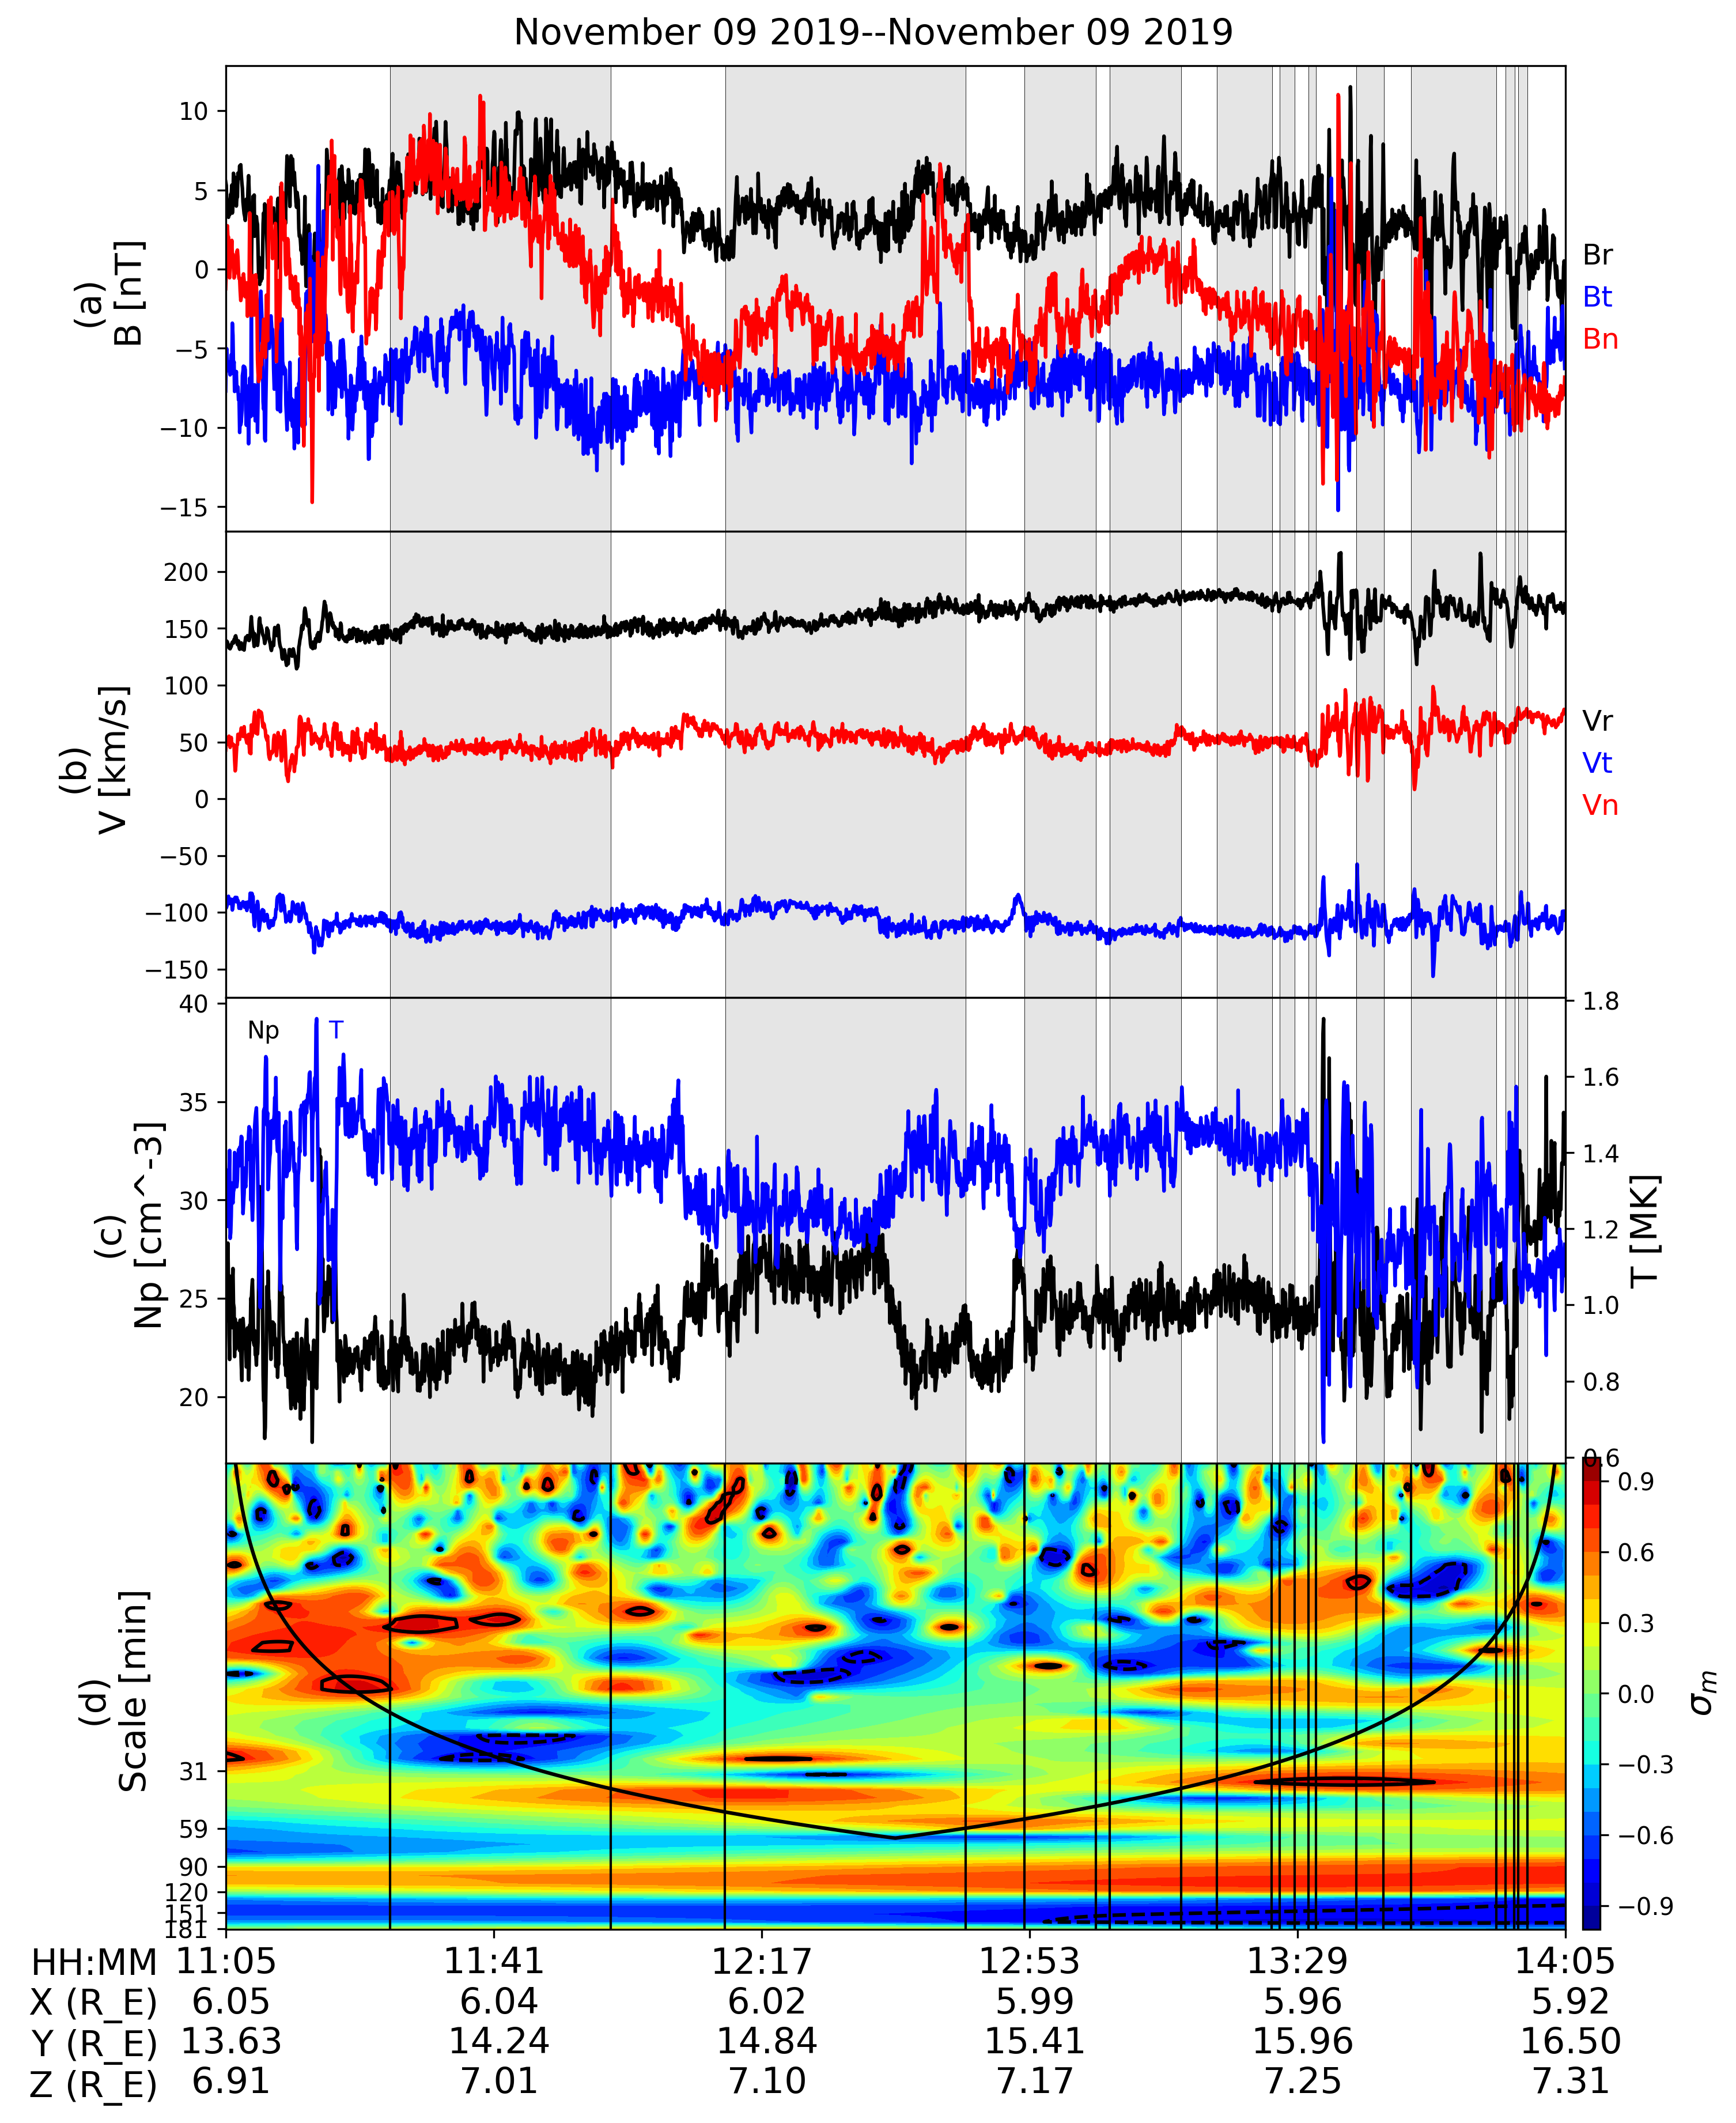
\includegraphics[width=0.9\textwidth]{Figures/Spectrograms/spectrogram_events_09112019_1105.png}
    \caption[Time series and spectrogram for 9 November 2019 with identified events overlaid]{Portion of the 9 November 2019 time series and reduced magnetic helicity spectrogram. The grey intervals representing events identified with wavelet analysis meeting the criteria $|\sigma_m|\geq 0.75$.}
    \label{fig:wavelet-spectrograms-interval}
\end{figure}


\section{Event categorization}\label{sec:wavelet-results}
There were 4260 events identified from the wavelet analysis in the magnetosheath across 1051 hours. For the solar wind, there were 3193 events identified across 676 hours via wavelet analysis. The occurrence rate for events in the solar wind from the wavelet method is about 4.7 events/hour and for the magnetosheath the corresponding rate is about 4.0 events/hour. Table  \ref{tab:regions-wavelet-summary} summarizes the events identified with the wavelet analysis algorithm.
\begin{table}
    \centering
    \caption{Summary table for identified events in the solar wind and magnetosheath via wavelet analysis as described in Section \ref{sec:wavelet-algorithm}.}
    % \begin{tabular}{rcccccc}
% \hline
%  & Hours  & Events &  Avg. duration &  Avg.    &  Avg. scale & Event rate \\
%  &           &           & [mins]   &  B [nT]      &  size [km]  & [\#/hour] \\
% \hline
% \textit{Solar wind}     & 676   &  3193  & 7.40 & 4.93  & 161241.93 & 4.723 \\
% \textit{Magnetosheath}  & 1051  &  4260  & 8.76 & 20.21 & 110801.05 & 4.053 \\
% \hline
% \end{tabular}

\begin{tabular}{rccc}
\hline
                        & Observation   & Events &  Event rate \\
                        & period [hrs]  &        &  [\#/hour]  \\
\hline
\textit{Solar wind}     & 676           &  3193  & 4.723 \\
\textit{Magnetosheath}  & 1051          &  4260  & 4.053 \\
\hline
\end{tabular}
    \label{tab:regions-wavelet-summary}
\end{table}

Properties of the magnetic structures are recorded during the identification process. Table \ref{tab:wavelet-stats} summarizes the statistical values for the identified events. The average duration of the events is 7.40 and 8.76 minutes for the solar wind and magnetosheath, respectively. In the solar wind, there are a large number of events with an average magnetic field of less than 10 nT, whereas in the magnetosheath there are relatively much fewer events with $\langle B\rangle < 10$ nT. The median magnetic field magnitude in the solar wind is 4.6 nT for events identified with wavelet analysis, and in the magnetosheath this number is 16.5 nT. As shown in Table \ref{tab:wavelet-stats}, the duration of the events has similar ranges for the two regions. However, for the scale sizes of the events in the magnetosheath, they range from $\sim$1507 km to 1.287$\times 10^6$ km, with a median and mean of 3.441$\times 10^4$ km, $\sim$5.4 $R_E$ and 1.108$\times 10^5$ km, $\sim$17.4 $R_E$, respectively. In the solar wind, the corresponding values are from 8975.2 km to 2.107$\times 10^6$ km, and a median (mean) of 5.444$\times 10^5$ (1.612$\times 10^5$) km, $\sim$8.5 (25.3) $R_E$. It is important to note that the calculations of scale size cannot be considered as physically reliable as the calculations from the GS-based method since the specificity of the wavelet analysis identification method relies on factors such as data segment length and choice of wavelet basis, in addition to the calculations being done in the spacecraft frame of reference.
\begin{table}
    \centering
    \caption[Statistical values for the physical quantities of structures identified with wavelet analysis]{Statistical values for the physical quantities of the structures identified in the magnetosheath (top) and solar wind (bottom) with wavelet analysis.}
    \begin{tabular}{lccccc}
\hline
       & Minimum & Maximum & Mean & Median & Std. Dev. \\
\hline
Duration [min]         & 0.517    & 59.221             & 8.761              & 2.617     & 12.6 \\
Velocity [km/s]        & 13.653   & 567.539            & 220.381            & 214.361   & 75.4 \\
Temperature [10$^6$ K] & 0.601    & 31.611             & 2.908              & 2.200     & 2.3  \\
$<B>$ [nT]             & 2.344    & 85.790             & 20.213             & 16.473    & 12.2 \\
Scale size [km]        & 1506.944 & 1.287$\times 10^6$ & 1.108$\times 10^5$ & 3.441$\times 10^4$ & 1.6$\times 10^5$ \\

\hline \hline

Duration [min]         & 0.560    & 59.221             & 7.402              & 2.400     & 10.6 \\
Velocity [km/s]        & 235.264  & 664.001            & 367.580            & 342.591   & 87.4 \\
Temperature [10$^6$ K] & 0.114    & 16.946             & 2.600              & 0.685     & 3.4 \\
$<B>$ [nT]             & 0.543    & 29.372             & 4.935              & 4.576     & 2.5 \\
Scale size [km]        & 8975.252 & 2.107$\times 10^6$ & 1.612$\times 10^5$ & 5.444$\times 10^4$ & 2.4$\times 10^5$ \\

\hline
\end{tabular}

    \label{tab:wavelet-stats}
\end{table}

Table \ref{tab:wavelet-event-summary} categorizes the events identified via wavelet analysis based on meeting certain MHD criteria. Over half of the events in the solar wind have characteristics of static flux ropes ($|\sigma_m|\geq 0.75$, $|\sigma_c|\leq 0.3$, $\sigma_r<0$), whereas in the magnetosheath there are fewer events (approximately one-third) that meet these criteria.
\begin{table}
    \centering
    \caption{Summary table of events meeting certain MHD criteria for events identified via wavelet analysis in the magnetosheath and solar wind.}
    \label{tab:wavelet-event-summary}
    \begin{tabular}{rcc}
\hline
{} & Solar wind & Magnetosheath \\
\hline
$|\sigma_m|\geq 0.75$                        & 3193 & 4260  \\
$|\sigma_m|\geq 0.75$, $|\sigma_c|\leq 0.3$  & 1821 & 2490  \\
$|\sigma_m|\geq 0.75$, $\sigma_r<0$          & 2156 & 2468  \\
$|\sigma_m|\geq 0.75$, $|\sigma_c|\leq 0.3$, $\sigma_r<0$ & 1144 & 1567 \\
\hline
%\multicolumn{3}{c}{$^c$in the magnetosheath and solar wind.}
\end{tabular}
\label{tab:wavelet-event-summary}

% sw_eventCount + msh_eventCount
\end{table}
The distribution of the reduced cross helicity and residual energy for all identified events in the solar wind and magnetosheath is shown in Figure \ref{fig:mhd_histogram-wavelet}. The histogram shows the averaged, reduced MHD quantities of the events identified by the wavelet method. Figure \ref{fig:mhd_histogram-wavelet} shows flatter distributions of reduced cross helicity $\sigma_c$ in the magnetosheath than in the solar wind. The reduced cross helicity distribution maintains a peak around $\sigma_c=0$ in both regions in Figure \ref{fig:mhd_histogram-wavelet}, with the solar wind having a steeper shape. The reduced residual energy has a peak at $\sigma_r=-1$, with values that are nearly evenly distributed between $(-1,1)$.

\begin{figure}
    \centering
    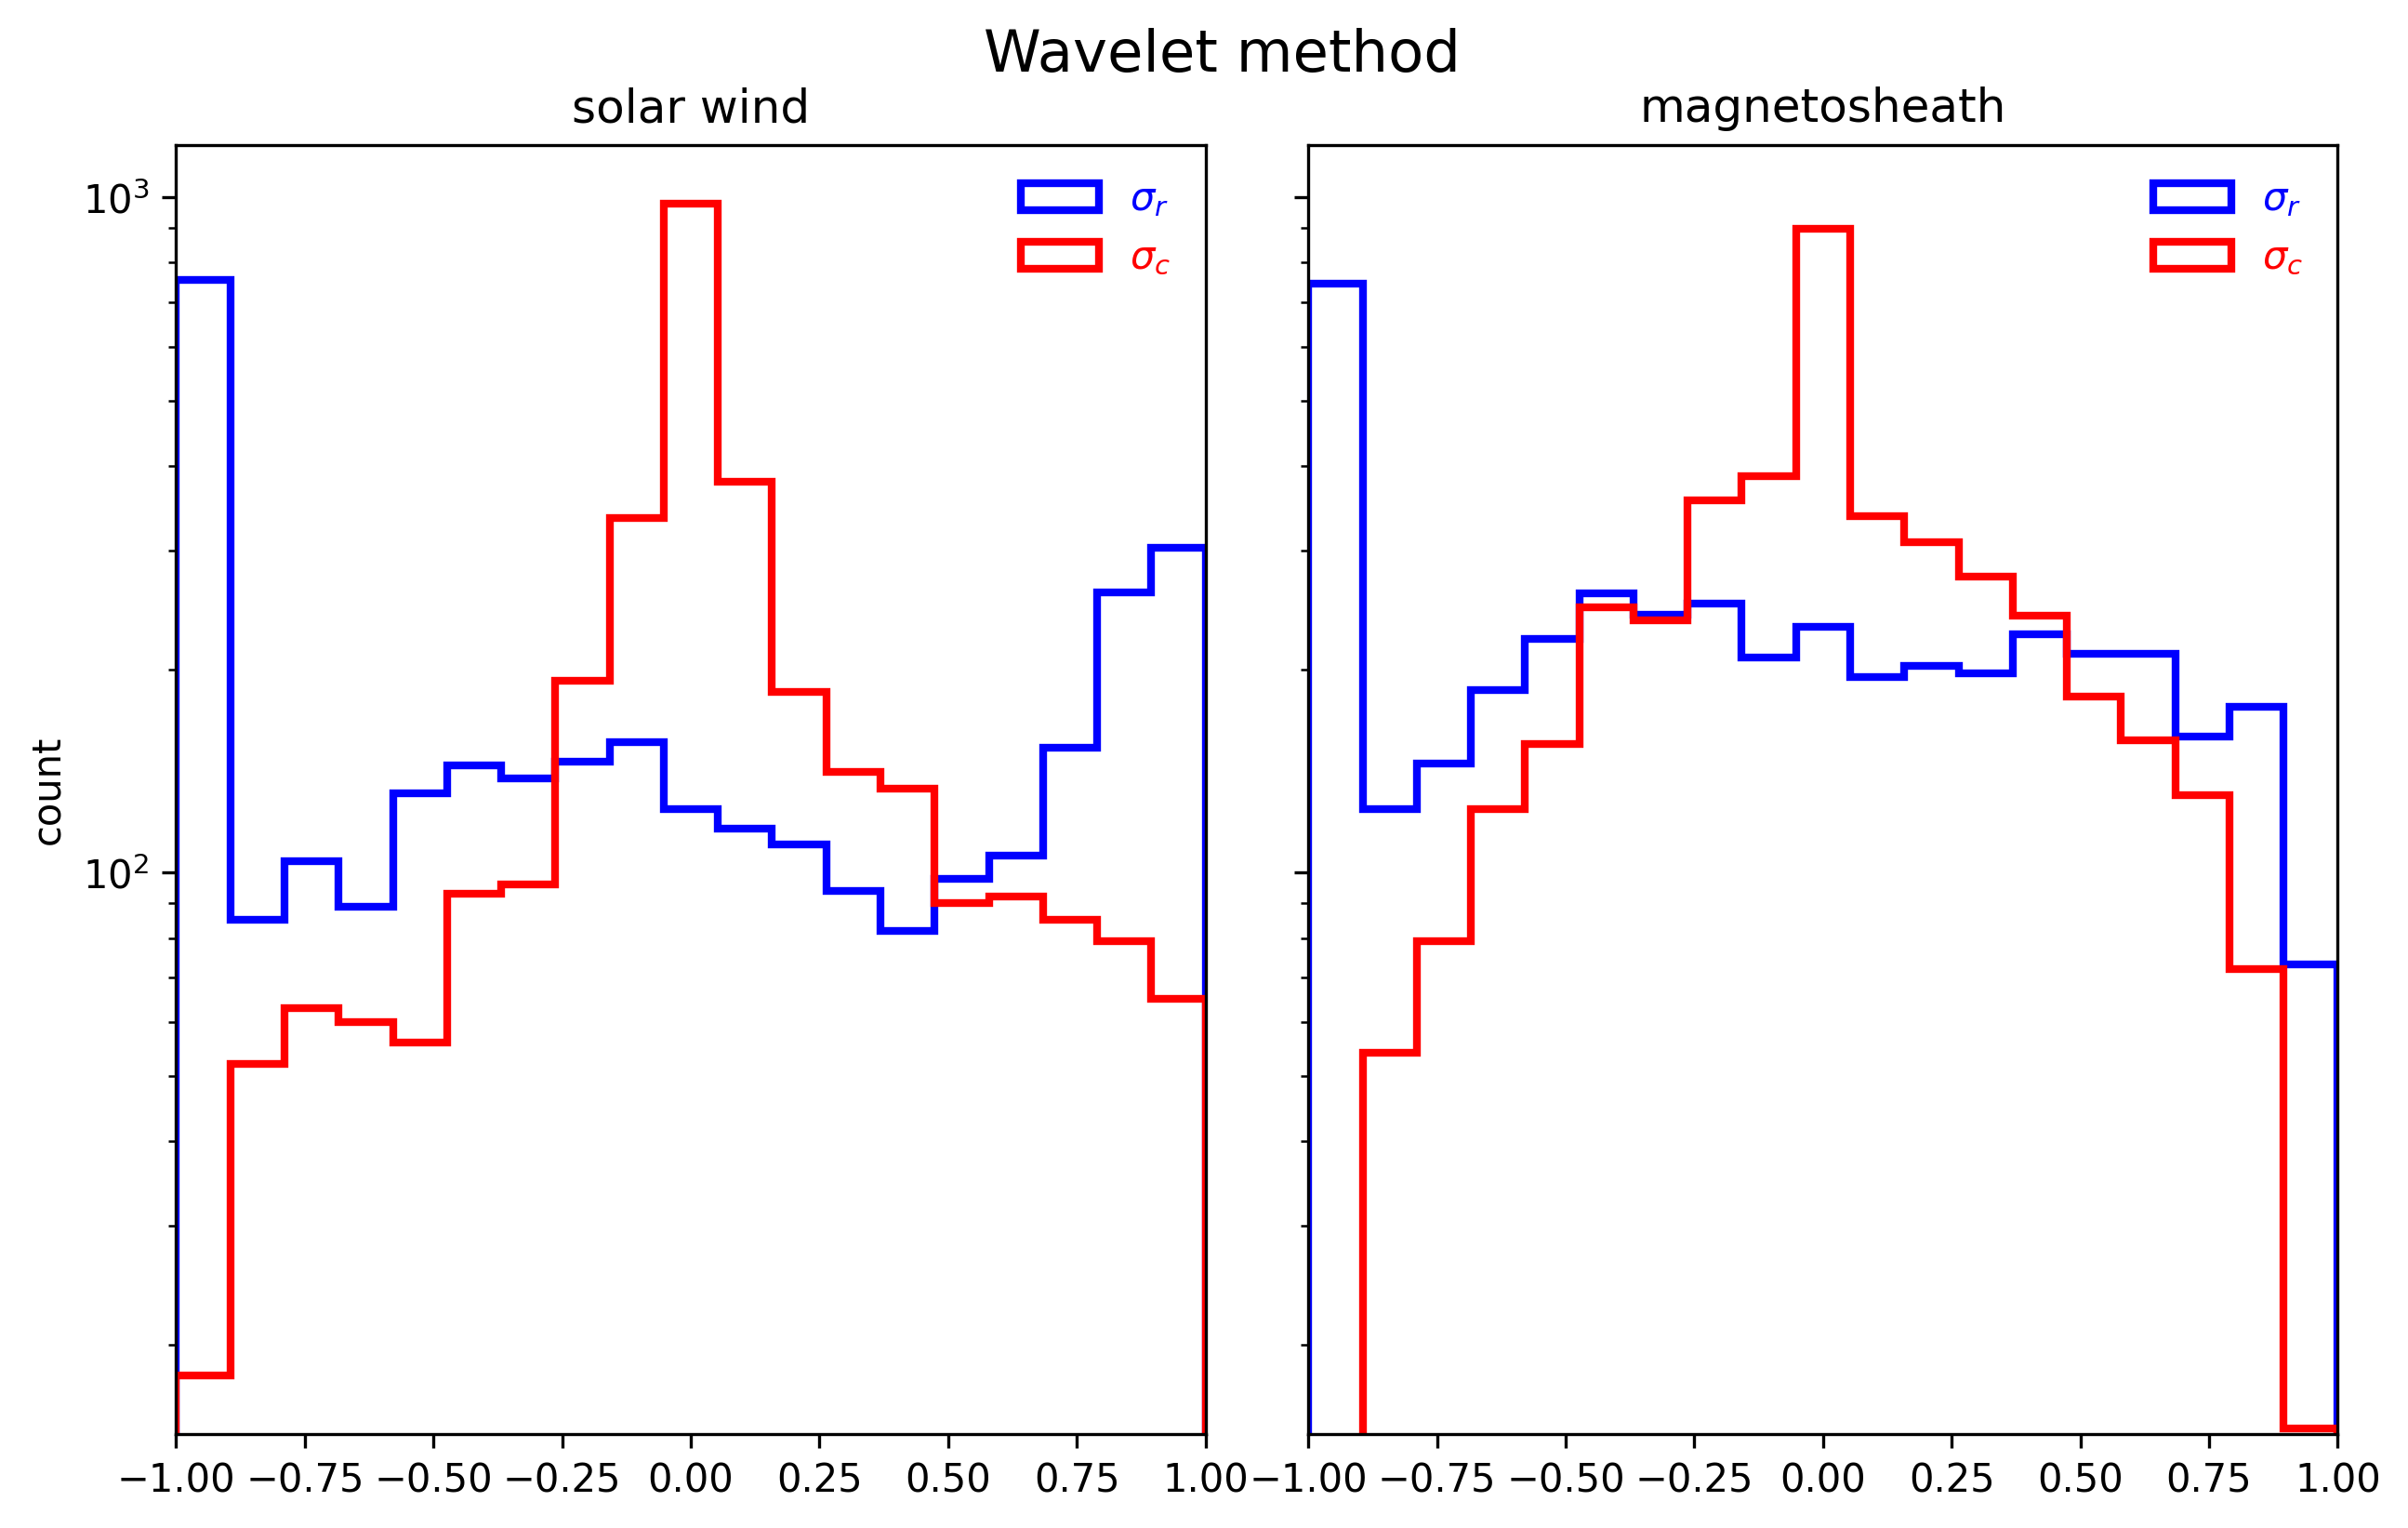
\includegraphics[width=\textwidth]{Figures/Histograms/sigr_sigc_wavelet.png}
    \caption[Reduced cross helicity and reduced residual energy for all events identified via wavelet analysis]{Histograms of reduced cross helicity $\sigma_c$ (red) and reduced residual energy $\sigma_r$ (blue) for all solar wind (left) and magnetosheath events (right) identified via the wavelet method.}
    \label{fig:mhd_histogram-wavelet}
\end{figure}